\chapter{The Game}
\section{What is the Mighty Map Crawler?}
This is  a cooperative dungeon crawling game for 1 to 6 players, which can be played by everyone without the need for a game master or expensive equipment. \\ All you need is a printer, a dry-erase-map (or a piece of paper), and time! The character progress is consistent across a campaign.\\ \\ Every player starts by creating a character according to the rules on page XXX.\\ After that, a scenario is selected, which consists of a short introductory text, a scenario goal and a \textit{dungeon map}(see section \ref{dungeon_map_section}). 

\section{Before you play}
Print the monster and equipment cards, which should be included in your download.

\section{The Dungeon Map\label{dungeon_map_section}}
In figure \ref{fig:scenariobasemap} you can see a simple scenario base map
\begin{figure}
	\centering
	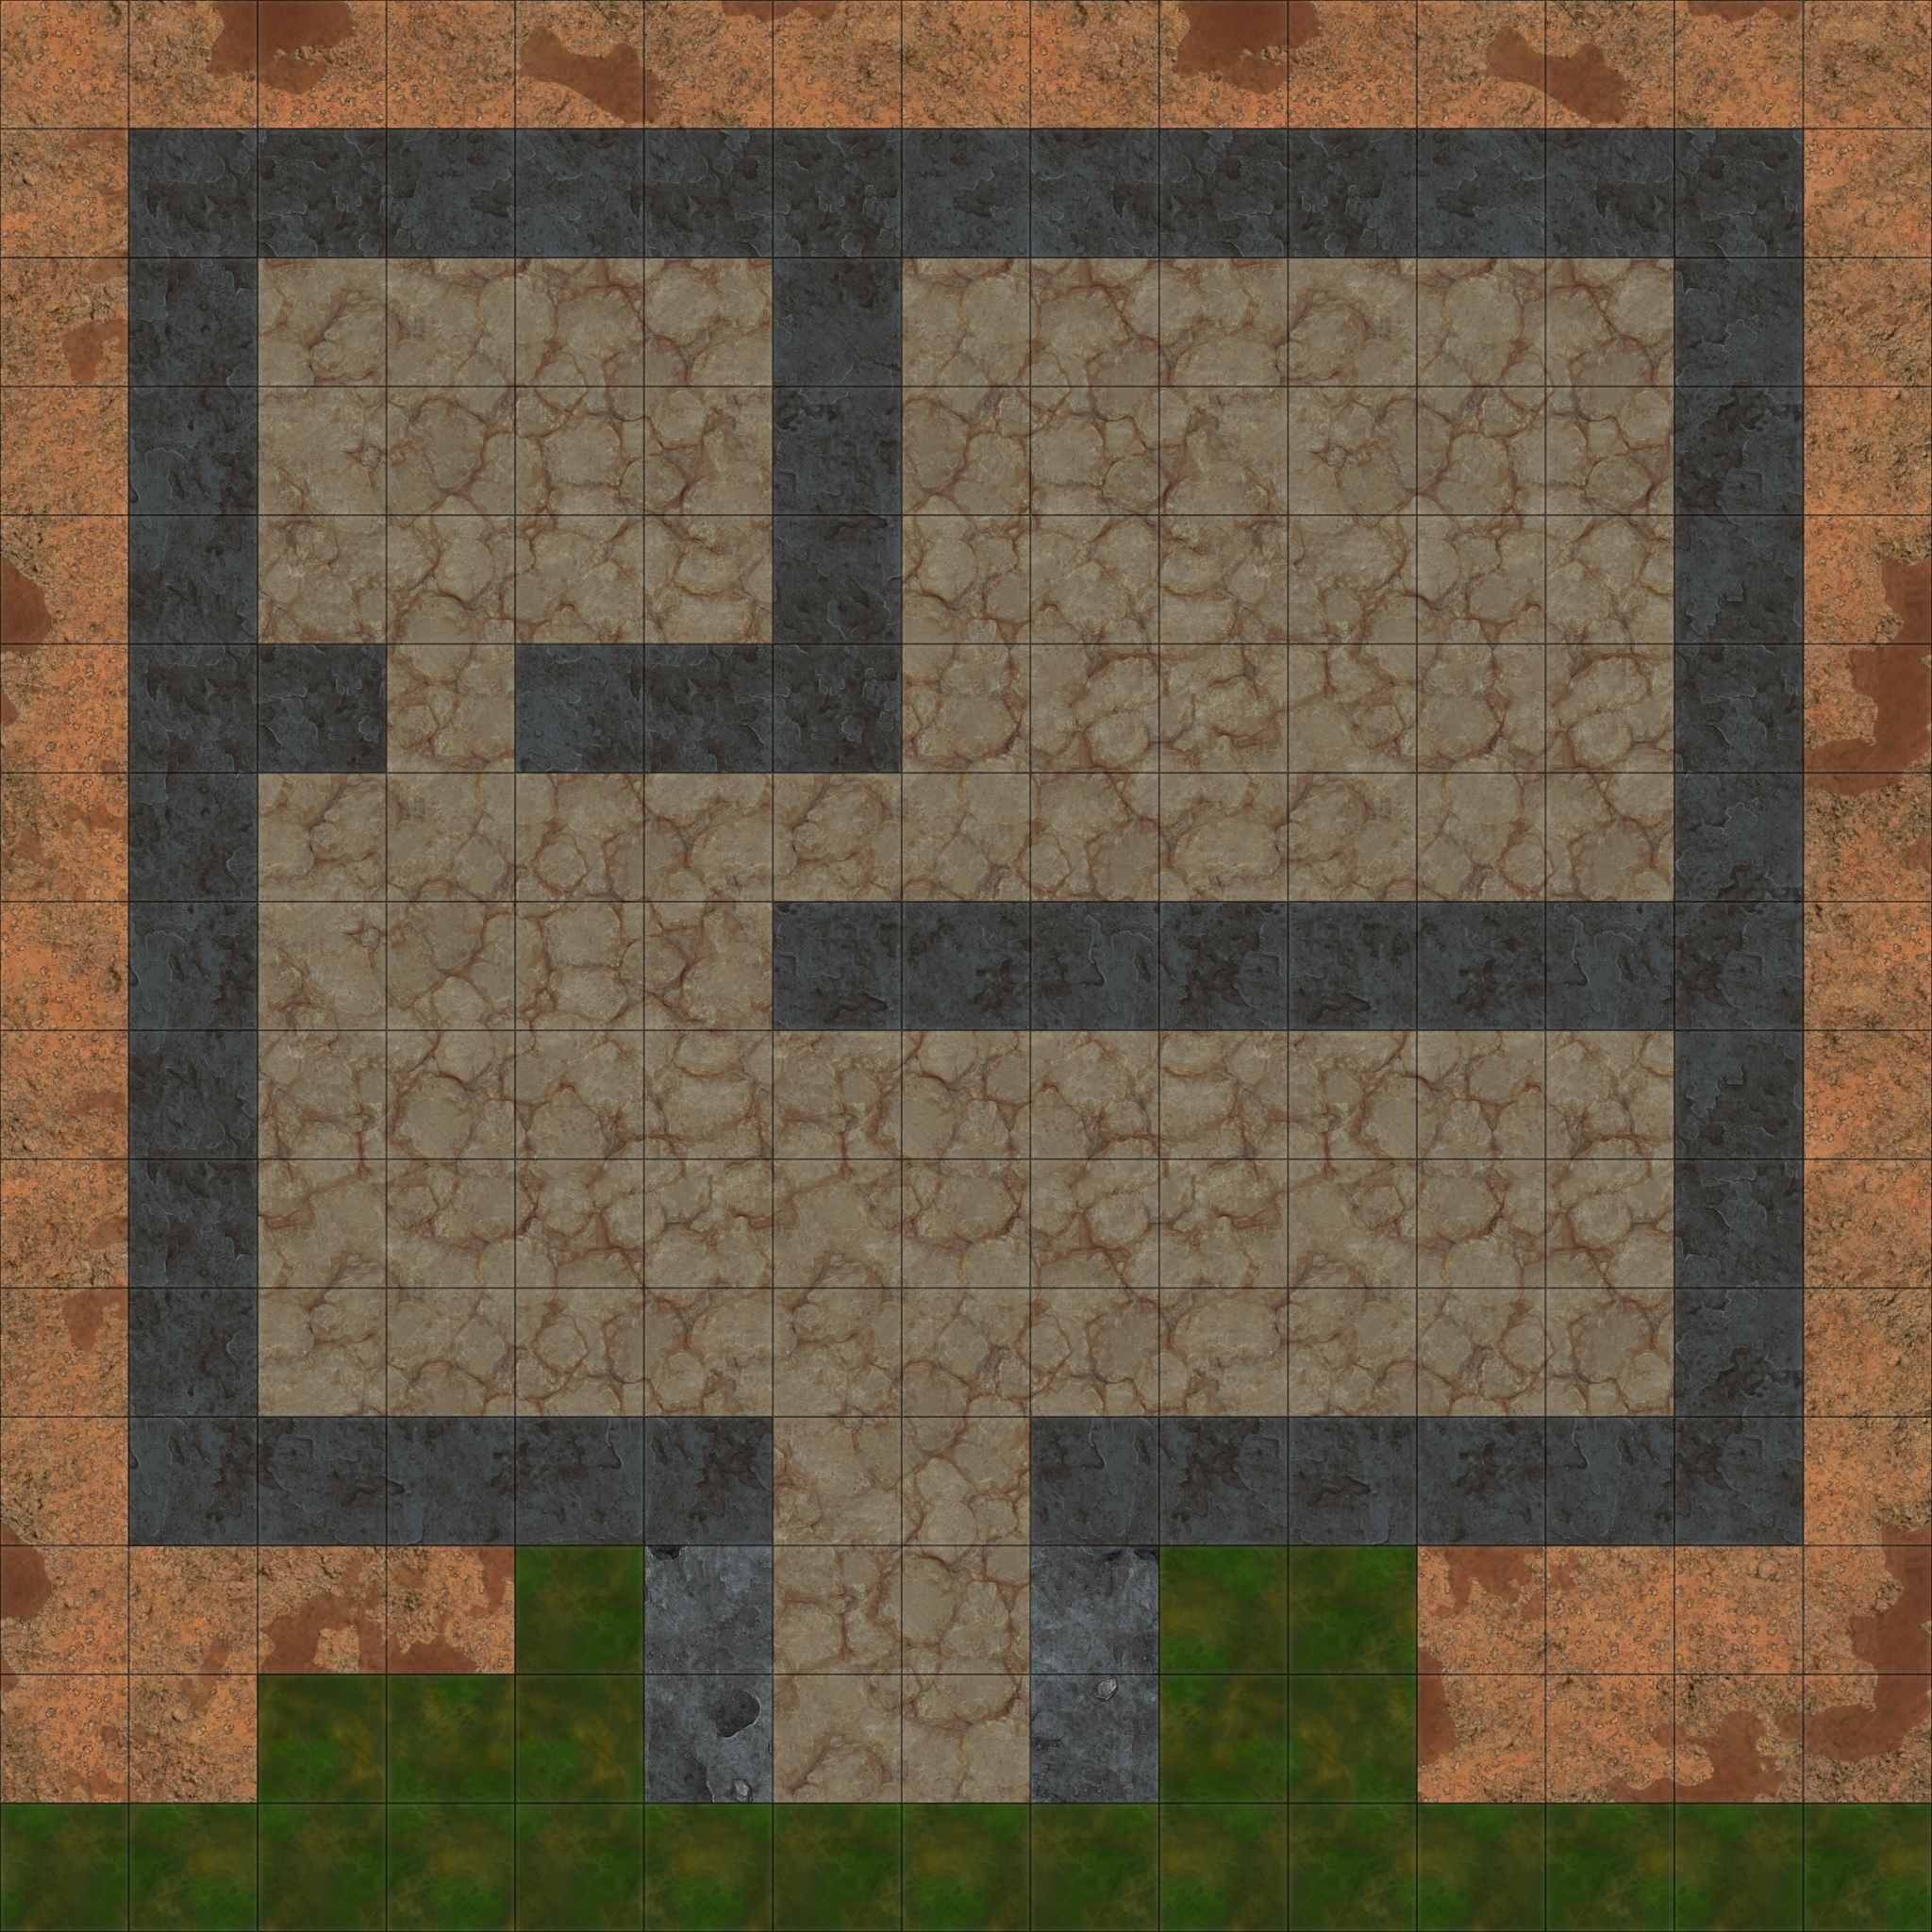
\includegraphics[width=0.7\linewidth]{TeX_files/ScenarioBaseMap}
	\caption{The first dungeon}
	\label{fig:scenariobasemap}
\end{figure}


\section{Monster Cards}
Your enemies in this game are monsters. Each monster has four stats: lifepoints (LP), movement range (M),attack range (R), and attack (A). Additionally, a monster can have \textit{conditional actions}, which are performed each time the requirements are met. 